%!TEX root = *.tex
%%%%%%%%%%%%%%%%%%
% カウンタのリセット
\setcounter{figure}{0}
% 問題文
円筒部分と漏斗部分からなる同形の2つの容器AとBの漏斗部分の先どうしをコックのついた細管でつないで,内部に単原子分子理想気体と液体を封入する.
容器A,Bはともに容積が$V_0$であり,
液体の体積は$V_1\,(V_1<V_0)$で温度によらず一定である.
液体の蒸気圧は無視できるものとする.
細管は十分に細く,細管部分の体積は無視できる.
細管内に液体が入っているときは,容器A,B内の気体は混ざらない.

はじめ,液体がすべて容器Aに入っている状態でコックを閉じ,容器Aを上に,容器Bを下にして鉛直に立てて置いた(図1(a);以下,状態(a)と呼ぶ).
このとき,容器A,B内の気体はどちらも圧力が$P_0$で絶対温度(以下,単に温度という)が$T_0$であった.
コックを開くと液体は少量ずつ容器B内に落下していき,
液体がほぼすべて落下してもまだ細管内に液体が残って容器A,B内の気体が分けられている状態(図1(b);以下,状態(b)と呼ぶ)になった.
その後,細管内の液体も容器B内に落下して容器A,B内の気体が混合されて,容器A,B内の気体は圧力,温度とも一様の状態(図1(c);以下,状態(c)と呼ぶ)になった.
なお,状態(b),(c)のおいて,液体の上面は水平になっていた.
液体の落下には十分に時間がかかり,状態(a)から(b)への変化において,
気体は十分ゆっくり変化する(準静的な変化をする)ものとする.
以下の設問に答えよ.


\begin{figure}[H]
  \centering
  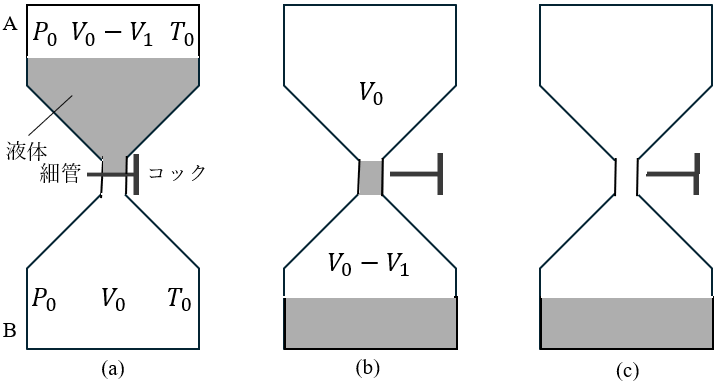
\includegraphics[width=.8\columnwidth]{../graphs/open_19_8_3-1.png}
  \caption{}
\end{figure}

\begin{enumerate}[\ajRoman{\arabic{enumi}}]
  \setlength{\leftskip}{-1zw}
  \setlength{\itemindent}{1zw}\setlength{\labelsep}{0.5zw}
  \setlength{\labelwidth}{1zw}\setlength{\leftmargin}{1zw}
  \setlength{\itemsep}{0.5\baselineskip}
  \item まず,容器内の気体の温度がつねに一定に保たれる場合を考える.
  \begin{enumerate}[(1)]
    \setlength{\leftskip}{-2zw}
    \setlength{\itemindent}{1zw}\setlength{\labelsep}{1zw}
    \setlength{\labelwidth}{1zw}
    \item 状態(a)において,容器A,B内の気体の物質量をそれぞれ$n_{\rm A},\,n_{\rm B}$とする.$n_{\rm A}$と$n_{\rm B}$の比を$V_0$と$V_1$を用いて表せ.
    \item 状態(b)において,容器A,B内の気体の圧力をそれぞれ$P_{\rm A},\,P_{\rm B}$とする.$P_{\rm A}$と$P_{\rm B}$の比を$V_0$と$V_1$を用いて表せ.
    \item 状態(a)から状態(b)に変化する間の,容器A,B内のそれぞれの気体の状態変化の様子を,縦軸に体積$V$,横軸に圧力$P$を取ったグラフ($P$--$V$グラフ)上に描け.ただし,圧力$P_0$,$P_{\rm A}$,$P_{\rm B}$を縦軸に明記し,また,容器A内の気体の変化は実線で,容器B内の気体の変化は破線で示せ.
    \item 状態(a)から状態(b)に変化する間に,容器A内の気体が吸収した熱量を$Q_{\rm A}$,容器B内の気体が吸収した熱量を$Q_{\rm B}$とする.$\abs{Q_{\rm A}}$と$\abs{Q_{\rm B}}$の大小関係を答えよ.また,設問\ajRoman{1}(3)で描いたグラフの中で,面積の値が$\abs{Q_{\rm A}+Q_{\rm B}}$のエネルギー量と等しくなる領域を,斜線で塗りつぶして示せ.
    \item 状態(c)において,容器内の気体の圧力を求めよ. 
  \end{enumerate}
  \item 次に,装置全体を断熱材で包み,容器内の気体および液体が外部と熱のやり取りをしない場合を考える.液体の熱容量を$C$,状態(a)から(b)に変化する間の液体の落下による重力の位置エネルギー減少量を$E$,気体定数を$R$とする.容器の熱容量は無視できるものとする.
  \begin{enumerate}[(1)]
    \setlength{\leftskip}{-2zw}
    \setlength{\itemindent}{1zw}\setlength{\labelsep}{1zw}
    \setlength{\labelwidth}{1zw}
    \item 状態(a)から(b)に変化する間について述べた次の文章中の空欄\BrankNo{(ア)}$\sim$\BrankNo{(エ)}に当てはまる最も適切な式を,以下の選択肢\ctext{1}$\sim$\ctext{12}から選んで答えよ.
    
    \vspace{\baselineskip}
    \quad 液体の落下による重力の位置エネルギー減少量$E$の一部は,いったん液体の落下の運動エネルギーになるが,液体分子どうしの衝突や液体分子と容器の壁との衝突などによりすべて熱エネルギーに変わるものとする.その熱量を$Q$とする.さらにそのうち,容器A,B内の気体に伝わる熱量を$Q_{\rm A},\,Q_{\rm B}$とする.また,状態(a)から(b)に変化する間の,容器A,B内の気体および液体の内部エネルギー変化量をそれぞれ$\Delta U_{\rm A},\,\Delta U_{\rm B},\,\Delta U_{\rm L}$,容器A,B内の気体が外部にした仕事をそれぞれ$W_{\rm A},W_{\rm B}$とする.\\
    \quad 容器A,B内の気体および液体について,それぞれエネルギー保存則(熱力学第一法則)を表す式を立てると,
    \begin{align*}
      \text{容器A}&: \quad Q_{\rm A} = \BrankNo{(ア)} \\
      \text{容器B}&: \quad Q_{\rm B} = \BrankNo{(イ)} \\
      \text{液体}&: \quad Q-(Q_{\rm A}+Q_{\rm B})=\Delta U_{\rm L} \\
    \end{align*}
    となる.一方,容器内の液体と気体の全体についてエネルギー保存則を表す式を立てると,
    \begin{align*}
      E = \BrankNo{(ウ)} 
    \end{align*}
    となる.つまり,$E-Q=\BrankNo{エ}$が成り立つ.\\
    【選択肢】\\
    \ctext{1}\quad $\Delta U_{\rm A}+W_{\rm A}$ \hspace{\stretch{1}}
    \ctext{2}\quad $\Delta U_{\rm A}-W_{\rm A}$ \hspace{\stretch{1}}
    \ctext{3}\quad $\Delta U_{\rm B}+W_{\rm B}$ \hspace{\stretch{1}}
    \ctext{4}\quad $\Delta U_{\rm B}-W_{\rm B}$ \\
    \ctext{5}\quad $\Delta U_{\rm A}+U_{\rm B}$ \hspace{\stretch{1}}
    \ctext{6}\quad $\Delta U_{\rm A}+U_{\rm B}+U_{\rm L}$ \hspace{\stretch{1}}
    \ctext{7}\quad $\Delta W_{\rm A}+W_{\rm B}$ \hspace{\stretch{1}}
    \ctext{8}\quad $\Delta -(W_{\rm A}+W_{\rm B})$ \\
    \ctext{9}\quad $\Delta U_{\rm A}+U_{\rm B}+W_{\rm A}+W_{\rm B}$ \hspace{\stretch{1}}
    \ctext{10}\quad $\Delta U_{\rm A}+U_{\rm B}-W_{\rm A}-W_{\rm B}$ \hspace{\stretch{1}}\mbox{}\\
    \ctext{11}\quad $\Delta U_{\rm A}+U_{\rm B}+U_{\rm L}+W_{\rm A}+W_{\rm B}$ \hspace{\stretch{1}}
    \ctext{12}\quad $\Delta U_{\rm A}+U_{\rm B}+U_{\rm L}-W_{\rm A}-W_{\rm B}$ \hspace{\stretch{1}}\mbox{}
    \item 状態(a)から(b)に変化する間の,容器A内の気体の圧力変化を$\Delta P_{\rm A}$,容器B内の気体の圧力変化を$\Delta P_{\rm B}$とする.$\Delta P_{\rm B}$を$\Delta P_{\rm A},\,V_0,\,V_1,\,E,\,\Delta U_{\rm L}$を用いて表せ.
    \item 状態(c)における容器内の気体の温度を,$n_{\rm A},\,n_{\rm B},\,C,\,R,\,E,\,T_0$を用いて表せ.
  \end{enumerate}
\end{enumerate}


%%%%%%%%%%%%%%%%%%